\documentclass[11pt]{article}
\usepackage[utf8]{inputenc}
\usepackage[ngerman]{babel}

\usepackage{amsmath,amsthm,amssymb,amsfonts}

\usepackage{graphicx}

\usepackage{float}
\usepackage{tikz}

\usepackage{fancyhdr} % For headers and footers
\usepackage{geometry}
\usepackage{listings}
\usepackage{hyperref}
\hypersetup{
    linkcolor=blue,     
    urlcolor=cyan,
}

\geometry{
    a4paper, % Change this if you intend to print on a different paper size, such as letter paper.
    left=20mm,
    right=20mm,
    top=30mm,
    bottom=30mm,
}

\newcount\colveccount
\newcommand*\colvec[1]{
        \global\colveccount#1
        \begin{pmatrix}
        \colvecnext
}
\def\colvecnext#1{
        #1
        \global\advance\colveccount-1
        \ifnum\colveccount>0
                \\
                \expandafter\colvecnext
        \else
                \end{pmatrix}
        \fi
}

\title{Dynamik - Drehimpuls (Rotation)}
\author{Emil Staikov}
\date{14. Juni 2021}

\begin{document}
\maketitle
\section{Definition}
% BILD -> sin erklären!!!! 
\begin{figure}[H]
        \centering 
        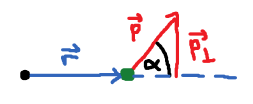
\includegraphics{abb/7-rotation-drehimpuls/drehimpuls.png}
        \caption{Definition des Drehimpulses}
\end{figure}
Für einen Massepunkt mit Impuls $\vec{p} = m\vec{v}$ im Abstand $\vec{r}$ von der Rotationsachse definieren wir den Drehimpuls $\vec{L}$, $[L] = \frac{kg\cdot m^2}{s}$, mit 
\begin{equation*}
        |\vec{L}| = |\vec{r}||\vec{p}_\bot | = |\vec{r}||\vec{p}|\sin \alpha 
\end{equation*}
Also als das Produkt aus der Länge des Radius und dem Betrag der zum Radius senkrechten Komponente des Impulses des Massepunkts. $\alpha$ ist der von $\vec{r}$ und $\vec{p}$ aufgespante Winkel, auch als $\angle \vec{r} \vec{p}$ geschrieben. \\\\
$\vec{L}$ hat als Vektor natürlich auch eine Richtung. $\vec{L}$ steht senkrecht zu $\vec{r}$ und $\vec{v}$, damit gibt es aber immernoch zwei mögliche Richtungen für $\vec{L}$. Wenn man mit der rechten Hand in Richtung von $\vec{r}$ zeigt und die Finger in Richtung von der zu $\vec{r}$ senkrechten Komponente von $\vec{p}$ (also in Richtung von $\vec{v}_T$) aufrollt, so zeigt der ausgestreckte Daumen in Richtung von $\vec{L}$. \\\\
Für mehr Massepunkte ergibt sich der Gesamtdrehimpuls als Summe der Drehimpulse der einzelnen Massepunkte. 


\section{Zusammenhang mit Größen der Rotationsbewegung}
Wir formen die Definition um
\begin{align*}
        |\vec{L}| &= |\vec{r}||\vec{p}|\sin \angle \vec{r} \vec{p} &|\textit{ Definition des Impulses} \\
        &= |\vec{r}||m\vec{v}|\sin \angle \vec{r} \vec{p} &|\textit{ Masse ist stets positiv} \\
        &= |\vec{r}|m|\vec{v}|\sin \angle \vec{r} \vec{p} &|\textit{ Definition der Tangentialgeschwindigkeit } v_T \\
        &= |\vec{r}|mv_T &|\textit{ Zusammenhang von Tangential- und Winkelgeschwindigkeit, } v_T = |\vec{r}|\omega \\
        &= |\vec{r}|m|\vec{r}|\omega &|\textit{ Umordnung der Terme}\\ 
        &= m|\vec{r}|^2\omega &|\textit{ Definition des Trägheitmoments eines Massepunkts } I = m|\vec{r}|^2 \\
        &= I\omega
\end{align*}
Der Zusammenhang $\vec{L} = I \omega$ gilt auch für beliebig viele Massepunkte und für arbiträre, starre Körper. Das Trägheitmoment ist entsprechend zu berechnen bzw. anzupassen. 


\section{Der Drehimpulserhaltungssatz}
Wie für die bisherigen Erhaltungssätze betrachten wir die Änderung der Erhaltungsgröße, in diesem Fall dem Drehimpuls, und formen um 
\begin{align*}
        \frac{\Delta \vec{L}}{\Delta t} &= \frac{\Delta \vec{r}\vec{p}}{\Delta t} &\textit{ Radius wird als konstant angenommen} \\
        &= \vec{r}\frac{\Delta \vec{p}}{\Delta t} &\frac{\Delta \vec{p}}{\Delta t} = \vec{F} \textit{ (s. Impuls-Skript)} \\ 
        &= \vec{r}\vec{F} &\textit{ Definition des Drehmoments} \\
        &= \vec{M}
\end{align*}
Für mehr Massepunkte, bzw. für beliebige, starre Körper und verschiedene wirkende Drehmomente gilt allgemein
\begin{equation*}
        \frac{\Delta \vec{L}}{\Delta t} = \sum \vec{M_{ext}}
\end{equation*}
Damit schließen wir auf den \\
\textbf{Drehimpulserhaltungssatz:} In jedem Inertialsystem gilt 
\begin{equation*}
        \sum \vec{M_{ext}} = 0 \implies \frac{\Delta \vec{L}}{\Delta t} = 0 \text{, also } \vec{L} = const. 
\end{equation*}
Hierbei ist $\sum \vec{M_{ext}}$ die Summe aller von außen auf das System wirkenden Drehmomente. Innere Drehmomente heben sich nach Newtons drittem Axiom in Inertialsystem stets auf. \\
Nach Komponentenzerlegung folgt aus der Beziehung zu den Größen der Rotationsbewegung 
\begin{equation*}
        L_x = I_x\omega_x = const. \quad\quad L_y = I_y\omega_y = const. \quad\quad L_z = I_z\omega_z = const. 
\end{equation*} 
Die Winkelgeschwindigkeit kann in ihre Komponenten zerlegt werden, das Trägheitsmoment muss jedoch für jede Achse einzeln berechnet werden. \\\\
Es bleiben sowohl Betrag als auch Richtung von $\vec{L}$ erhalten, wenn insgesamt kein äußeres Drehmoment wirkt, in IJSO-Aufgaben geht es jedoch meistens nur um betragliche Änderungen oder Vorzeichenänderungen (s. Beispiele). Damit reicht es meistens aus nur eine Komponente des Drehimpulses zu betrachten, das entspricht praktisch einer skalaren Größe. 


\section{Beispiele}
\textbf{Drehstuhl mit Gewichten:} Eine Person sitzt auf einem Drehstuhl und hat in beiden Händen jeweils ein $5kg$ Gewicht. Mit beiden Gewichten nah am Körper, also $10cm$ entfernt von der Rotationsachse, dreht sie sich mit einer halben Umdrehung pro Sekunde, also $\omega_1 = \pi \frac{1}{s}$. Mit welcher Geschwindigkeit $\omega_2$ dreht sich die Person, wenn sie beide Arme ausstreckt, sodass die Gewichte $1m$ Abstand von der Rotationsachse haben? Es wird angenommen, dass die Person genau auf der Achse steht, also selbst ein Trägheitmoment von $0 m^2kg$ hat. \\\\ 
Wir vernachlässigen Luftreibung und nehmen an, dass das Lager im Stuhl ideal ist. Also wirkt dort ebenfalls keine Reibungskraft. Auf das System wirken damit keine äußeren Drehmomente, der Drehimpuls bleibt erhalten. Wir bezeichnen die Masse der Gewichte mit $m = 5kg$, den Abstand am Anfang mit $r_1 = 0.1m$ und den Abstand am Ende mit $r_2 = 1m$. Vor dem Ausstrecken der Arme finden wir 
\begin{equation*}
        L = I_1\omega_1 = (mr_1^2 + mr_1^2)\omega_1 = 2mr_1^2\omega_1 = \frac{\pi}{10} \frac{kg\cdot m^2}{s}
\end{equation*}
Nach dem Ausstrecken vergrößert sich das Trägheitsmoment auf $I_2 = 2mr_2^2 = 10 m^2kg$, gerade haben wir $L = \frac{\pi}{10} \frac{kg\cdot m^2}{s}$ errechnet
\begin{align*}
        L &= I_2\omega_2 \\
        \iff \omega_2 &= \frac{L}{I_2} = \frac{\frac{\pi}{10} \frac{kg\cdot m^2}{s}}{10 m^2kg} = \frac{\pi}{100} \frac{1}{s}
\end{align*}
Vor dem Ausstrecken hat die sich drehende Person noch eine halbe Umdrehung, also $180$ Grad in einer Sekunde zurückgelegt. Nach dem Ausstrecken sind es nur noch $1.8$ Grad! \\\\
Als Übung: Diese Aufgabe kann auch mithilfe von Energieerhaltung gelöst werden. \\\\
\textbf{Schlittschuhläufer:} Das Prinzip der letzten Aufgabe finden wir auch an anderer Stelle. Wenn wir das Eis als reibungsfrei annehmen, und die Reibung mit der Luft vernachlässigen, so bleibt der Drehimpuls eines Schlittschuläufers in einer Pirouette näherungsweise erhalten. Dieser wird schneller, je näher seine Gliedmaßen am Körper liegen, da dann sein Trägheitsmoment kleiner wird. Im Gegenzug erhöht sich dann seine Winkel- und Tangentialgeschwindigkeit. Wenn er seine Arme und Beine wieder ausstreckt, wird sein Trägheitmoment größer, und er wird wieder langsamer. \\\\


\end{document}